\section{Method}
\label{sec:method}

In this section, we present the architecture of \name, discuss the components involved in the system, and the various users (i.e., actors) interacting with the system. We also present the authentication workflow that allows a user to publish an object with a publisher and the verification workflow that allows a user to verify the authenticity of a published object. 

\subsection{Architecture}
\label{sec:arch}

\name provides authentication and verification of digital objects created by a user (i.e., {\em \owner}) using a trusted entity called {\em \TA} (\ta). Any application that can create an object also registers and authenticates with \ta (for example, a mobile camera app). Owners and publishers register and authenticate themselves with the \ta. A \reader can retrieve published objects from the \publisher's portal, and may request \ta to verify any published objects. Figure \ref{fig:arch} shows the architecture of \name. 

\begin{figure*}[htpb]
  \centering
  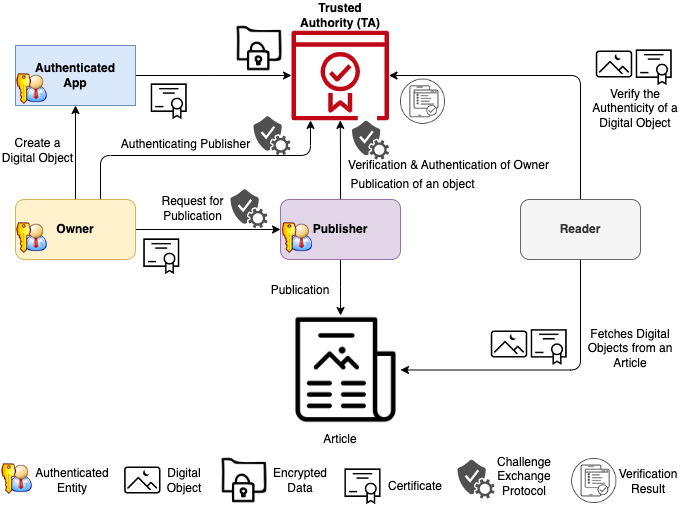
\includegraphics[scale=0.45]{architecture.png}
  \caption{Architecture of \name}
  \label{fig:arch}
\end{figure*}

While this architecture is similar to \cite{qqjs19}, we note that \name provides a mechanism for ensuring that any content-generation application can be made authentic and integrated with the proposed framework. And, \name simplifies the mutual authentication of an \owner and a \publisher (without a blockchain). 

\subsubsection{\bf Components of \name} 
The main components of \name are (1) \TA and (2) \AuthApp.

\begin{itemize}
  \item {\em \TA (\ta). } \
    \ta is similar to a Certificate Authority that issues and manages digital certificates to certify the ownership of public-key of named entities (e.g., website). Likewise, \ta is responsible for issuing and certifying public-private keys to registered entities. \ta is also responsible for issuing certificates to digital objects created by an \owner using an \authapp. Furthermore, \ta maintains the lineage of edits to a digital object. \ta allows the \publisher and \owner to mutually authenticate each other before publishing the owner's digital object. This process does not require any entity to share any confidential information explicitly. Finally, \ta verifies the certificate of a published object. 
  \item {\em \AuthApp. } \
    \AuthApp creates a digital object on request from an \owner. When the \owner requests (e.g., {\em clicks}) the \app to create an object, \app submits the created object to the \ta along with the credentials of the \app and the \owner for certification.
\end{itemize}

\subsubsection{\bf Actors of \name}
The main actors of \name are \owner, \publisher, and \reader. 

\begin{itemize}
  \item {\em \Owner. } \
    \Owner is an authenticated user of \ta and is responsible for the creation (or edits) of a digital object and publishing the digital object with a \publisher. 
  \item {\em \Publisher. } \
    \Publisher is an authenticated user of \ta and is responsible for publishing a digital object in its portal. In addition, the \publisher makes the certificate available for all published images in the portal. 
  \item {\em \Reader. } \
    \Reader can verify the published object's authenticity and lineage with the \ta. 
\end{itemize}

\subsection{Workflows}
\label{sec:workflows}

In this section, we discuss the primary workflows of \name.
% (1) creating a digital object, (2) publishing a digital object, and (3) verifying a published object.

\subsubsection{Creating a Digital Object}
\label{sec:new-object}

Figure \ref{fig:creation} shows the creation workflow. \Owner requests \authapp to create a new digital object (or save the edits performed on an existing digital object). \App then sends a certificate request to \ta with the name of the object, its payload (i.e., contents), and the identity of the \owner. If the object has lineage (i.e., the object is edited from an existing object), the \app includes the identity of the parent object and the certificate of the parent object in the request. \ta verifies authentication of the \app and the owner. Subsequently, if the lineage is part of the message, \ta verifies the certificate of the parent object. Finally, \ta issues a certificate for the object. 

\begin{figure}[htpb]
  \centering
  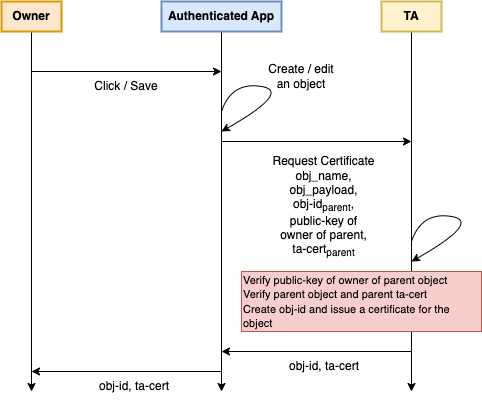
\includegraphics[scale=0.45]{creation.png}
  \caption{Creation of a digital object}
  \label{fig:creation}
\end{figure}

\subsubsection{Publishing a Digital Object}
\label{sec:pub-object}

% \begin{figure*}[htpb]
%   \centering
%   \begin{subfigure}[b]{.48\textwidth}
%     \centering
%     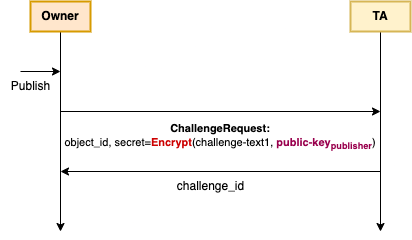
\includegraphics[scale=0.45]{challenge1.png}
%     \caption{Challenge creation}
%     \label{fig:challenge1}
%   \end{subfigure}%
%   \begin{subfigure}[b]{.48\textwidth}
%     \centering
%     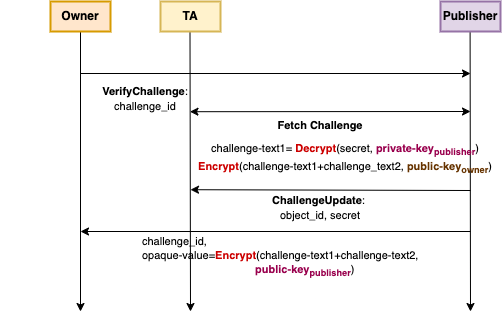
\includegraphics[scale=0.45]{challenge2.png}
%     \caption{Challenge exchange}
%     \label{fig:challenge2}
%   \end{subfigure}
%   \begin{subfigure}[b]{.48\textwidth}
%       \centering
%       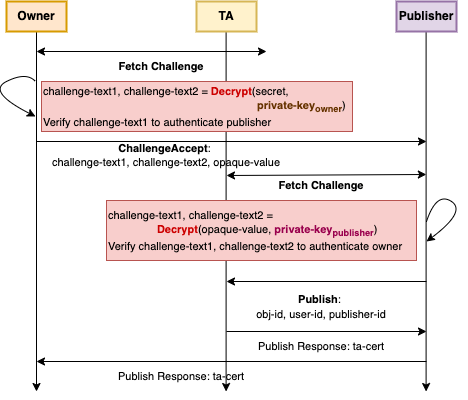
\includegraphics[scale=.45]{challenge3.png}
%       \caption{Challenge verification}
%       \label{fig:challenge3}
%     \end{subfigure}
%   \cprotect\caption{Publication of a digital object using a challenge protocol}
%   \label{fig:challenge}
% \end{figure*}

To publish a digital object, \owner and \publisher execute a challenge protocol modeled based on the Diffie-Hellman Key Exchange Protocol \cite{dh-key-exchange}.\footnote{We would like to note that there are many different implementations possible for the challenge protocol, including the implementation where the \owner and \publisher do not communicate directly. In our design, we let the \owner and the \publisher securely communicate while participating in the challenge protocol to authenticate each other mutually.} The protocol ensures mutual authentication of the \owner and \publisher before the publication of the digital object. 
%Figure \ref{fig:challenge} outlines the protocol.

\paragraph{Step 1: Challenge Creation}

An \owner initiates a challenge with the \ta when they decide to share an object. The challenge includes a random secret ({\em challenge-text1}) that is encrypted with the publisher's public key. \ta returns an ID for the challenge as shown in Figure \ref{fig:challenge1}. 

\begin{figure}[htpb]
  \centering
  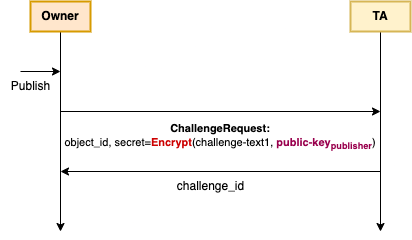
\includegraphics[scale=0.45]{challenge1.png}
  \caption{Challenge creation}
  \label{fig:challenge1}
\end{figure}

\paragraph{Step 2: Challenge Exchange} 

As shown in Figure \ref{fig:challenge2}, \owner sends the challenge ID to the \publisher. \Publisher retrieves the challenge from the \ta and decrypts the secret using the publisher's private key. Then, it creates a new random secret ({\em challenge-text2}) and appends it to the decrypted secret. Subsequently, it encrypts the combined secret with the owner's public key. \Publisher updates the combined secret at the \ta and replies to the \owner with an opaque value that the \owner should return to the \publisher for verification. This opaque value contains the value of the publisher's secret that is encrypted using the publisher's public key. (As a result, only the \publisher can decrypt this value.)

\begin{figure}[htbp]
  \centering
  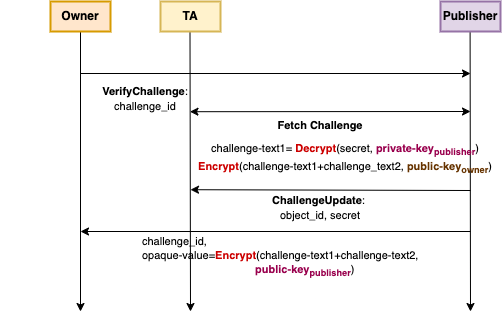
\includegraphics[scale=0.45]{challenge2.png}
  \caption{Challenge exchange}
  \label{fig:challenge2}
\end{figure}

\paragraph{Step 3: Challenge Verification}

In the final step (cf. Figure \ref{fig:challenge3}), \owner decrypts the secret in the challenge using its private key. \Owner authenticates \publisher if it sees {\em challenge-text1} in the message. When \owner decrypts the secret, it also gets the text that \publisher added in Step 2. To complete the authentication process, \owner sends a message to the \publisher that it accepted the challenge along with both the secrets and publisher's opaque value. \Publisher decrypts the opaque value and retrieves the original secrets. If the secrets match the texts in the message, \publisher authenticates \owner. 

\begin{figure}[htbp]
  \centering
  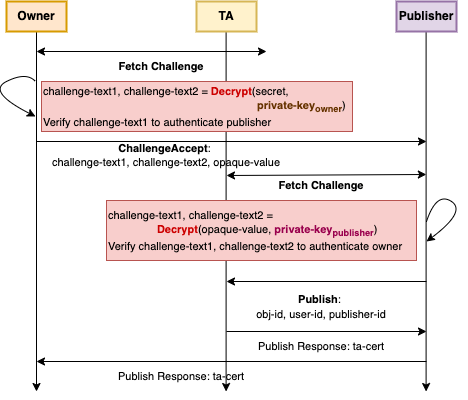
\includegraphics[scale=0.45]{challenge3.png}
  \caption{Challenge verification}
  \label{fig:challenge3}
\end{figure}

On successful authentication, \publisher requests the \ta to publish the object. The \ta validates provided information for publication and issues a signed certificate along with the owner's and publisher's public keys. Finally, the \publisher publishes the certified object in its portal.

\subsubsection{Verification of a Published Object}
\label{sec:verify}

A random \reader of the \publisher's portal can request verification of the digital objects published in the portal with the \ta. Figure \ref{fig:verification} outlines the verification process. First, \ta validates the digital signature of the certificate. Subsequently, \ta verifies that the public keys of the \owner and \publisher match. Finally, if the object has a lineage, \ta ensures the lineage is authentic and returns the validation result to the \reader. Thus, \name lets a \reader authenticate and verify the published objects without disclosing the \owner and any attributes associated with the \owner. 

\begin{figure}[htpb]
  \centering
  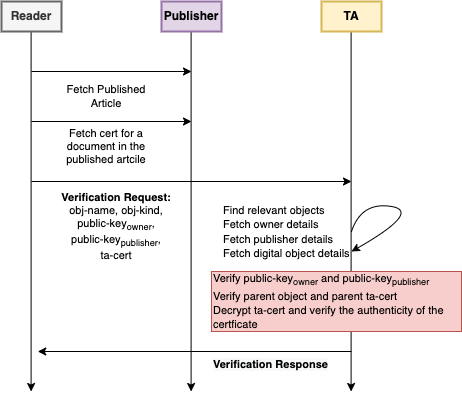
\includegraphics[scale=0.45]{verification.png}
  \caption{Verification of a published object}
  \label{fig:verification}
\end{figure}